Una rete è composta dall'hardware (computer, cavi), che permette di inviare una serie di bit da un nodo all'altro, che dal software, che permette di far assumere significato a questi bit e trasmettere un messaggio da un nodo a un qualsiasi altro nodo.

Per passare dai bit ai servizi di un software bisogna risolvere svariati problemi, ciascuno dei quali può essere inquadrato come appartenente a uno strato.

\section{Architettura a strati}
    Concettualmente immaginiamo un messaggio discendere dal mittente fra i diversi strati che lo codificano e decompongono, fino a spedirlo tramite il mezzo di comunicazione. Il destinatario farà risalire poi il messaggio attraverso gli stessi strati, ma in maniera inversa, quindi decodificandolo e ricomponendolo.
    
    Inoltre ogni strato offre un servizio allo strato superiore, e usa un servizio offerto dallo strato inferiore.
    
\section{Il modello OSI}
    Nonostante non sia stato usato a pieno perché surclassato da altri modelli, è un'ottima base per capire il funzionamento di un'architettura di rete a strati. È composto da sette livelli, ognuno dei quali definisce un particolare aspetto delle attività che servono per far muovere i dati sulla rete.
    
    \begin{figure}[h]
        \centering
        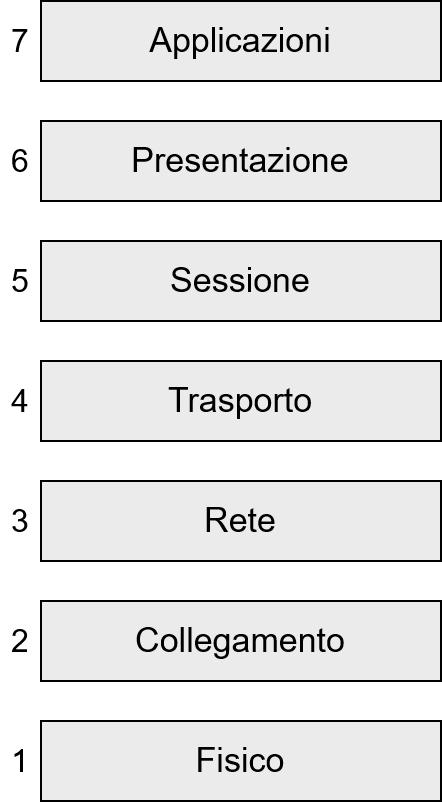
\includegraphics[width=0.33\textwidth]{img/strati_osi.png}
        \caption{I sette strati del modello OSI.}
        \label{fig:img1}
    \end{figure}
    
    Chiaramente ogni strato ha un'\textbf{interfaccia} che lo collega a quello precedente e a quello successivo. Questa interfaccia definisce quali servizi deve offrire allo strato sottostante e di quali può usufruire facendo riferimento allo strato superiore.
    
    Possiamo avere una serie di nodi intermedi nei tre stati più bassi (possiamo pensare a un mezzo fisico che non comunica direttamente col mezzo fisico di arrivo ma utilizza una serie di intermediari).
    
    Due livelli uguali di nodi diversi sono detti \textbf{peer}. La comunicazione fra due peer è detta peer-to-peer o p2p.
    
    \subsubsection{Organizzazione degli strati}
        I sette strati possono essere concettualmente divisi in tre gruppi:
        \begin{itemize}
            \item Gli \textbf{strati 1, 2, 3 (fisico, collegamento e rete)} sono strati per il supporto di rete, e hanno a che fare con le problematiche del mezzo fisico.
            
            \item Gli \textbf{strati 5, 6 e 7 (sessione, presentazione e applicazioni)} sono per il supporto all'utente, e permettono interoperabilità per sistemi che usano software diversi fra loro.
            
            \item Lo \textbf{strato 4 (trasporto)} collega i due gruppi sopra descritti.
        \end{itemize}
        
        Gli strati alti sono quasi sempre implementati in software, mentre gli strati bassi in un misto di hardware e software, tranne per lo strato fisico che è quasi sempre implementato quasi interamente in hardware.
    
    \subsection{Incapsulamento}
        Un aspetto importante della comunicazione dei dati del modello OSI è l'incapsulamento: il livello \textit{n} riceve dal livello \textit{n-1} un pacchetto di informazioni contenente sia i dati che l'header. Tuttavia i livelli più bassi non sanno niente dell'intestazione dei livelli più alti, e considerano l'intero pacchetto come un inseme unico di dati.
        
\newpage
\section{Strati del modello OSI}
    Qui descriveremo brevemente le funzioni di tutti gli strati del modello OSI.

    \subsection{Strato 1: Fisico}
        Deve tradurre la sequenza di bit nei segnali elettrici opportuni da inviare sul mezzo fisico. Gestisce le componenti meccaniche ed elettriche del mezzo trasmissivo.
        
        Per svolgere il suo compito deve avere a che fare con:
        \begin{itemize}
            \item \textbf{Caratteristiche fisiche dell'interfaccia e del mezzo trasmissivo.}
            
            \item \textbf{Rappresentazione dei bit.} Ossia come il valore 0 e il valore 1 sono codificati con i segnali da spedire sul mezzo trasmissivo.
            
            \item \textbf{Velocità di spedizione.} In altre parole, definisce quanto il segnale che rappresenta un bit deve durare (meno dura e maggiore è la velocità di spedizione).
            
            \item \textbf{Sincronizzazione dei bit.} Per una corretta lettura dei bit è necessario che il clock del mittenete e quello del destinatario siano sincronizzati.
            
            \item \textbf{Configurazione del collegamento.} La connessione del nodo al mezzo trasmissivo può essere punto-punto o multipunto.
            
            \item \textbf{Topologia.}
            
            \item \textbf{Flusso di dati.} Lo strato fisico definisce anche il tipo di comunicazione (simplex, half-duplex, duplex).
        \end{itemize}
        
    \subsection{Strato 2: Collegamento}
        Si occupa di varie problematiche fra cui correzione di errori; rende la trasmissione di pacchetti fra un nodo e l'altro affidabile. Deve avere a che fare con:
        \begin{itemize}
            \item \textbf{Framing.} Divide il flusso di bit che arriva dallo strato di rete e che deve essere spedito in blocchi, detti \textit{frame}.
            
            \item \textbf{Indirizzi fisici.} Se il destinatario è all'interno della stessa rete, nell'intestazione viene inserito il suo indirizzo fisico. Se è su un'altra rete, viene inserito l'indirizzo fisico del nodo che collega la rete corrente a un'altra rete.
            
            \item \textbf{Controllo di flusso.} Se le velocità di trasmissione e ricezione dei due nodi non sono in accordo, il flusso viene regolato per evitare un sovraccarico.
            
            \item \textbf{Controllo degli errori.} Permette di individuare i frame danneggiati e quindi di ritrasmetterli.
            
            \item \textbf{Controllo per l'accesso.} Quando il mezzo trasmissivo è multipunto, questo strato ha il compito di controllare quale nodo ha accesso al mezzo.
        \end{itemize}
        
        La comunicazione nello strato di collegamento avviene fra due frame successivi. Sia l'atto della trasmissione che i frame coinvolti vengono chiamati \textit{hop}.
        
    \subsection{Strato 3: Rete}
        Ha il compito di far arrivare il pacchetto di dati dal mittente al destinatario in una interrete, facendoli passare, se necessario, attraverso altre reti. Da ciò si evince che due nodi sulla stessa rete, per comunicare, non avranno bisogno dello strato di rete.
        
        Questo strato deve avere a che fare con:
        \begin{itemize}
            \item \textbf{Indirizzamento logico.} L'indirizzamento fisico non basta quando due nodi non sono sulla stessa rete. L'indirizzamento adeguato non dipende dalle componenti fisiche e si chiama indirizzamento logico.
            
            \item \textbf{Routing.} Quando più reti sono connesse fra di loro, i nodi che le connettono sono chiamati router. Il compito dello strato di rete è proprio di gestire questo meccanismo di routing.
        \end{itemize}
        
    \subsection{Strato 4: Trasporto}
        Si occupa della consegna di un messaggio da un processo mittente a un processo destinatario. Lo strato di rete non riconosce i pacchetti come appartenenti allo stesso messaggio, mentre lo stato di trasporto aggiunge questa logica, rendendo la fruizione del messaggio affidabile.
        
        Lo strato di collegamento deve avere a che fare con:
        \begin{itemize}
            \item \textbf{Indirizzamento dei processi.} Abbiamo visto che lo strato di rete si occupa di far giugnere i pacchetti al nodo destinatario. Lo strato di trasporto si occupa invece di smistare i pacchetti ai processi corretti. Questo tipo di meccanismo, che permette di distinguere fra i processi, viene chiamato indirizzo di servizio o di porta.
            
            \item \textbf{Segmentazione e riassemblaggio.} I singoli messaggi devono essere divisi in segmenti, ognuno dei quali contiene un numero di sequenza che permette il riassemblaggio una volta giunti a destinazione.
            
            \item \textbf{Controllo della connessione.} In una comunicazione senza connessione, i pacchetti vengono spediti in maniera indipendente l'uno dall'altro. Lo strato di trasporto offre invece una comunicazione con connessione, dove il mittente crea una connessione con lo strato di trasporto del destinatario prima di inviare i pacchetti contenenti i dati veri e propri. La connessione viene chiusa una volta che l'intero messaggio accordato è stato spedito.
            
            \item \textbf{Controllo del flusso.} Stavolta questo tipo di controllo avviene sui processi terminali, anziché sul mezzo di comunicazione come avviene per lo strato di collegamento.
            
            \item \textbf{Controllo degli errori.} Anziché operare sull'intero canale come in precedenza, si occupa della consistenza del messaggio scambiato fra i processi terminali.
        \end{itemize}
        
    \subsection{Strato 5: Sessione}
        Esso stabilisce, manitiene e sincronizza l'interazione fra i sistemi che comunicano. Le sue funzionalità sono:
        \begin{itemize}
            \item \textbf{Controllo del dialogo.} Permette a due sistemi, anche eterogenei, di comunicare.
            
            \item \textbf{Sincronizzazione.} Lo strato di sessione offre la possibilità ai processi di avere dei punti di controllo. Per esempio nell'invio di un messaggio da 1000 pagine, è opportuno controllare la corretta trasmissione ogni 100, così da diminuire l'eventuale numero di pagine da ritrasmettere.
        \end{itemize}
        
    \subsection{Strato 6: Presentazione}
        Si occupa di problematiche relative alla sintassi e alla semantica delle informazioni che devono essere trasmesse. Le sue funzionalità sono:
        \begin{itemize}
            \item \textbf{Traduzione.} Le informazioni di alto livello come il codice devono essere tradotte in sequenze di bit. Poiché diversi sistemi usano diversi schemi di codifica, queste differenze devono essere superate per permettere interoperabilità. Deve quindi essere usato un formato standard di rete, conversione che viene fatta dallo strato di presentazione.
            
            \item \textbf{Cifratura.} Nel mittente potrebbe avvenire una cifratura dei dati da spedire, cosa che richiederebbe poi una decifratura nello strato di presentazione del destinatario.
            
            \item \textbf{Compressione.}
        \end{itemize}
        
    \subsection{Strato 7: Applicazioni}
        Si occupa di fornire i servizi di rete all'utente finale, e comprende funzioni fra cui:
        \begin{itemize}
            \item \textbf{Terminale virtuale.} Un'emulazione del terminale del nodo remoto.
            
            \item \textbf{Gestione file.} Permette accesso e modifica di file da remoto.
            
            \item \textbf{Servizi di posta.} Permette lo scambio di messaggi elettronici fra utenti di una rete.
            
            \item \textbf{Servizi directory.}
        \end{itemize}
        
\section{La suite di protocolli TCP/IP}
    Gli strati di questa suite di protocolli non coincidono con quelli del protocollo OSI, in quanto sono stati sviluppati contemporaneamente, quando i secondi ancora non erano uno standard. Inizialmente ve ne erano quattro: strato nodo-rete, di rete, di trasporto e delle applicazioni. Lo strato nodo-rete comprende le funzionalità che nel modello OSI sono comprese nello strato fisico e in quello di collegamento, mentre lo strato delle applicazioni ingloba le funzionalità degli strati di sessione, presentazione e applicazioni del modello OSI.
    
    Definiremo il modello TCP/IP come composto da cinque strati che chiameremo fisico, di collegamento, di rete, di trasporto e delle applicazioni e che possono essere messi in corrispondenza con gli equivalenti strati del modello OSI, sebbene gli ultimi tre strati del modello OSI corrispondano a uno solo nel modello TCP/IP.
    
    La differenza principale fra il modello OSI e quello TCP/IP è che in quest'ultimo abbiamo strati strutturati gerarchicamente, nel senso che uno strato alto può essere supportato da uno o più strati bassi. Questo rende la struttura meno rigida e meno opaca.
    
    Per lo strato di trasporto TCP/IP definisce tre protocolli: TCP (Transmission Control Protocol), UDP (User Datagram Protocol) e SCTP (Stream Control Transmission Protocol). Per lo strato di rete il protocollo principale è IP (Internet Protocol).
    
    \subsection{Strati 1 e 2: fisico e di collegamento}
        Per questi strati il modello TCP/IP non definisce nessun protocollo, bensì supporta tutti i protocolli proprietari definiti dalle reti nelle quali TCP/IP viene utilizzato.
        
    \subsection{Strato 3: Rete}
        Come abbiamo detto, in questo strato viene definito il protocollo IP (Internet Protocol), che fa uso di quattro protocolli di servizio: ARP, RARP, ICMP e IGMP.
        
        \subsubsection{Protocollo IP}
            Il protocollo IP fornisce il servizio basilare di consegna pacchetti da un nodo all'altro nell'interrete. Il protocollo così definito è senza connessione e inaffidabile, un servizio detto \textit{best-effort}.
            
            Questo protocollo trasporta i dati in pacchetti detti \textit{datagram}, in maniera indipendente l'uno dall'altro. Come abbiamo detto, il protocollo IP non offre funzionalità per ovviare ai problemi a cui possono essere soggetti i \textit{datagram}, come arrivo non in ordine, perdita o duplicazione dei pacchetti. Nonostante ciò, esso offre funzionalità considerevoli in maniera abbastanza efficiente per le reti per le quali deve funzionare. Ulteriori accortezze nel suo funzionamento possono essere aggiunte usandolo semplicemente come base.
            
        \subsubsection{ARP (Address Resolution Protocol)}
            Il protocollo ARP permette di tradurre gli indirizzi logici usati dal protocollo IP per individuare i nodi nella interrete in in indirzzi fisici.
            
        \subsubsection{RARP (Reverse Address Resolution Protocol)}
            Questo protocollo permette di eseguire l'operazione inversa, ossia di risalire all'indirizzo IP logico a partire da quello fisico. Tipicamente viene usato quando il PC viene acceso e scoprire il suo indirizzo IP a partire dall'hardware.
            
        \subsubsection{ICMP (Internet Control Message Protocol)}
            Il protocollo ICMP viene usato per il controllo della rete. Quando si verifica un errore viene inviato un messaggio ICMP all'utente.
            
        \subsubsection{IGMP (Internet Group Message Protocol)}
            Esso offre delle funzionalità per la trasmissione simultanea di un messaggio a un gruppo di destinatari.
            
    \subsection{Strato 4: Trasporto}
        Mentre il protocollo IP permette di trasportare i pacchetti da un computer mittente a uno destinatario, i protocolli TCP e UDP permettono di trasportare i pacchetti da un processo mittente a un processo destinatario.
        
        È stato poi introdotto il protocollo SCTP per supportare alcune applicazioni recenti.
        
        \subsubsection{UDP (User Datagram Protocol)}
            È un protocollo molto semplice, che rispetto a IP introduce l'uso delle porte per l'identificazione dei processi, un codice per la rilevazione di errori e informazioni relative alla lunghezza dei dati provenienti dagli strati superiori.
            
        \subsubsection{TCP (Transmission Control Protocol)}
            Esso fornisce un servizio di trasporto affidabile fra processi orientato al flusso. Quindi questo protocollo stabilisce una connessione fra i punti terminali prima di spedire dati.
            
            Il mittente divide il flusso di byte da spedire in pezzi detti segmenti, ognuno dei quali ha un numero di sequenza che ne preserva l'ordine. Vengono poi passati al destinatario all'interno di datagram IP, che li riceverà prima di ordinarli.
    
    \subsection{Strato 5: Applicazioni}
        È equivalente alla combinazione degli strati di sessione, presentazione e applicazioni del modello OSI.